
\begin{center}
	\Large\textbf{{\textcolor{black}{AGRADECIMIENTOS}}}
\end{center}Los autores desean expresar su agradecimiento a:

\vspace{2pc}

\begin{minipage}[c]{0.2\linewidth}
	\frame{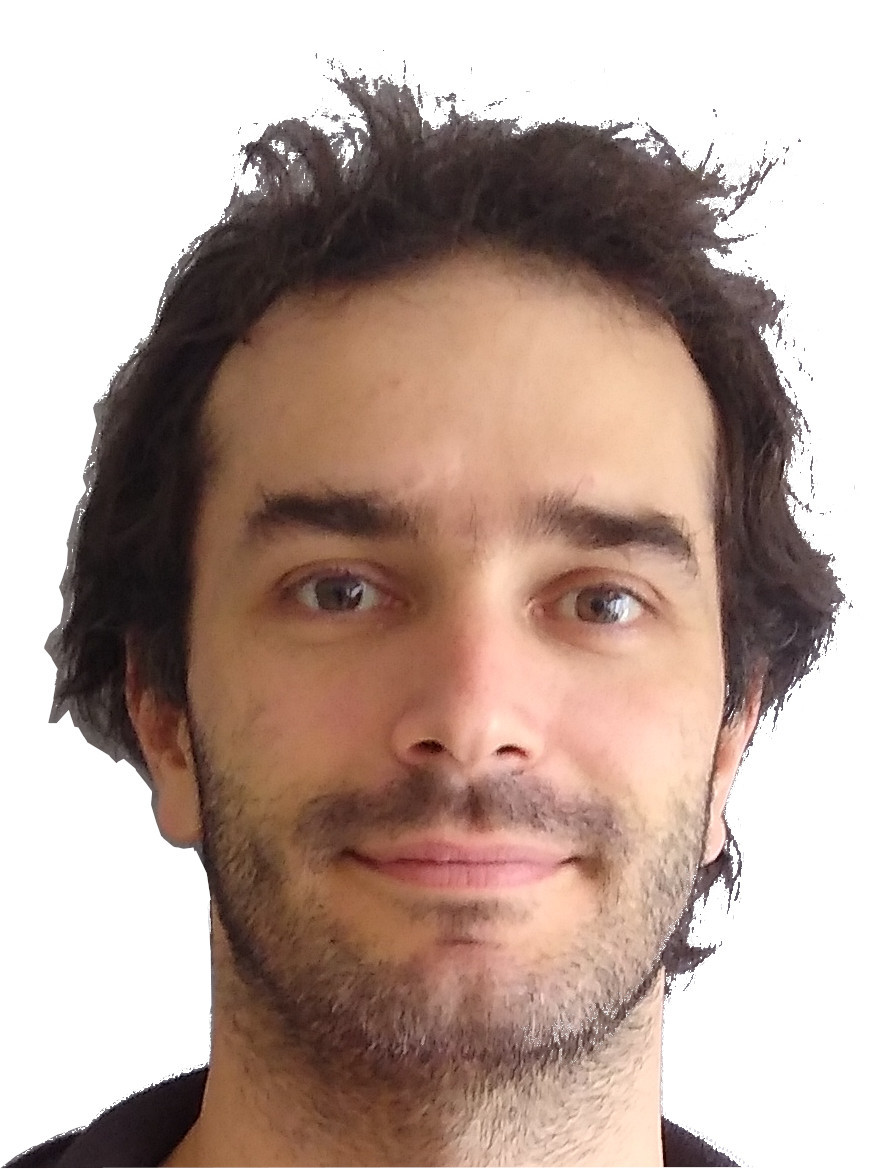
\includegraphics[width=.7\textwidth]{graficos/Foto_carnet_AGCV_Rojo.jpg}}
\end{minipage}
\hfill
\begin{minipage}[c]{0.7\linewidth}
	Ing. Rui Marques Rojo, investigador RPIDFA que forma parte del equipo de trabajo del Departamento de Propagación Acústica de la Dirección de Investigación de la Armada, por el montaje y puesta a punto de la plataforma Gitea con servicios para el desarrollo de código, que fuera extensamente utilizada en la realización del trabajo que aquí se documenta.  Asimismo, se deja constancia de sus valiosas sugerencias para la implementación de código en lenguaje Python.
\end{minipage}%\vfill

\vspace{2pc}
\clearpage
